%  LaTeX template for abstract submission for SAMO 2022
% 
% First name and name of the speaker.
\speaker{Philipp}{Eisenhauer}%
%  (put no space here)
% Title of the talk, capitalized.
\title{Robust decision-making under risk and ambiguity*}

% For each author, give the first name, family name, affiliation, and email.
% Ideally, the affiliation and email should fit on a single line.  
% No need to put the full snail mailing address.  
%  One line per author 
\author{ Maximilian }{Blesch}{Berlin School of Economics, Germany}{maximilianblesch@web.de}
\author{Philipp}{Eisenhauer}{University of Bonn, Germany}{peisenha@uni-bonn.de}


% Type your abstract here.
\abstract{%Include your abstract here. You can give references  like here \cite{ref1} or \cite{ref2}. 
%Recall that if you need to define your own macros, it is required to include your name in their definitions. \textbf{(1,000 words and 2 pages maximum)}
Individuals face ubiquitous uncertainties when faced with important decisions. For example, policymakers vote for climate change mitigation efforts facing uncertainty about future costs and benefits \cite{Barnett.2020} and individuals save parts of their current income to cover uncertain medical expenses in old age \cite{French.2014}. Economic models formalize the objectives, trade-offs, and uncertainties of such decisions and inform decision-making processes. However, the treatment of uncertainty is often limited to risk as the model induces a unique probability distribution over sequences of possible futures. There is no role for ambiguity about the true model \cite{Arrow.1951,Knight.1921} and thus no fear of model misspecification.\\

At the same time, it is common practice in economics to  estimate a subset of the model parameters outside the model and let the decision-makers inside the model treat these point estimates as-if they correspond to the true parameters.\footnote{See for example \cite{Berger.2015}, \cite{Blundell.2016}, \cite{Cagetti.2006}, \cite{Chiappori.2018}, \cite{DeNardi.2010}, \cite{Ejrnaes.2020},  \cite{Fernandez.2014}, \cite{French.2011}, \cite{Gourinchas.2002}, \cite{Huo.2020}, \cite{Scholz.2006}, \cite{Sommer.2016}, and  \cite{Voena.2015}.} This approach ignores any uncertainty in the first-step estimation and opens the door for model misspecification. As-if decision-makers, decision-makers who use the point estimates to inform decisions that would be optimal if the estimates were accurate, face the risk of serious disappointment about their decisions. The performance of as-if decisions often turns out to be very sensitive to model misspecification \cite{Smith.2006}. This danger creates the need for robust decision rules that work well over a whole range of different models instead of an as-if decision rule that is best for one particular model.\\

Figure \ref{Robust decisions}
 clarifies the notion of robust decision-making. It shows the performance of the as-if and a robust decision rule for different levels of model misspecification. The as-if decision rule is designed without fear of misspecification, using a single model to inform decisions. It thus performs very well if that model turns out to be true. However, its performance is susceptible to model misspecification and deteriorates rapidly in its presence. Robust decision rules account for such a possibility, and their performance is less affected. At some point, the robust approach outperforms the as-if alternative.\\
%
\begin{figure}[h!]\centering
	\caption{Models of decision-making}\label{Robust decisions}
	\scalebox{0.65}{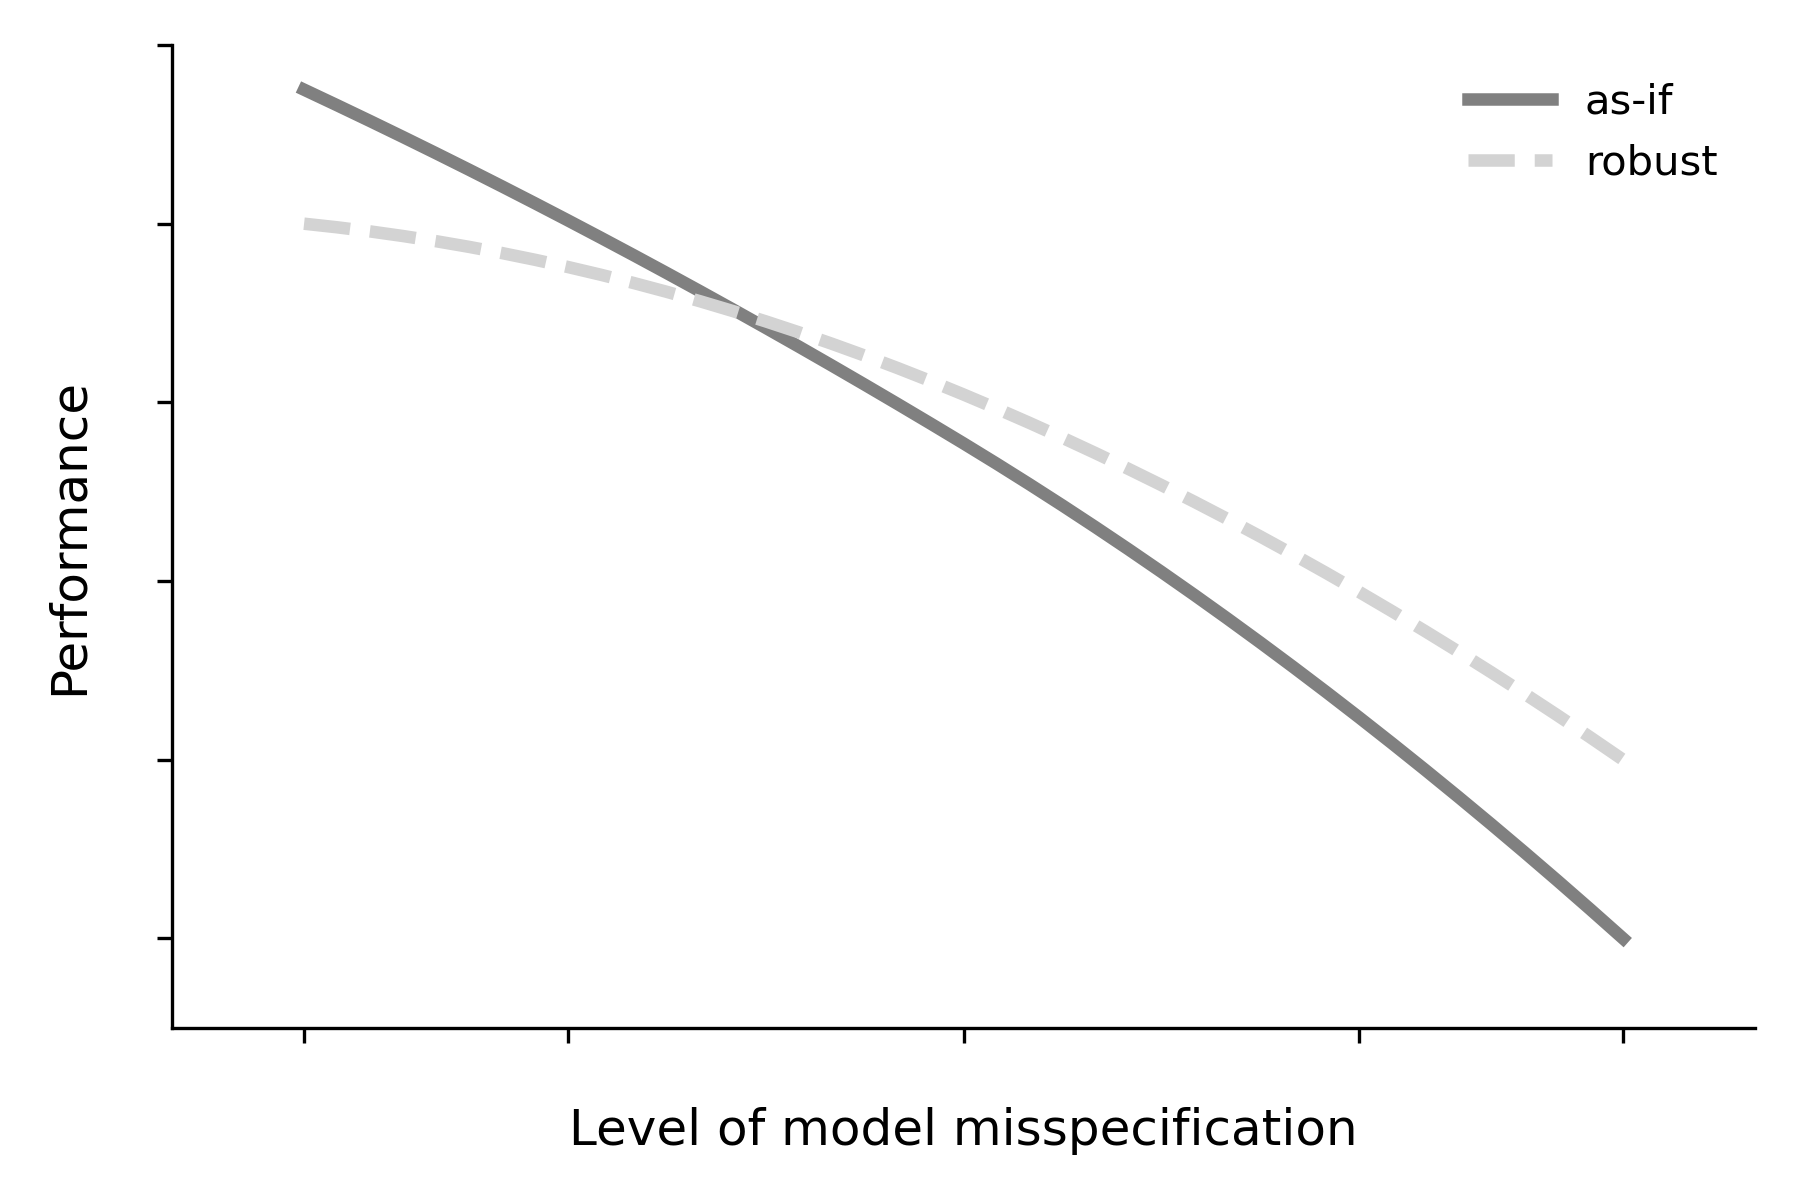
\includegraphics{fig-introduction-robust-performance-sw}}
\end{figure}%\FloatBarrier
%
We develop a framework to evaluate as-if and robust decision rules in a decision-theoretic setting by merging insights from the literature on data-driven robust optimization \cite{Bertsimas.2018} and robust Markov decision processes \cite{Ben-Tal.2009} with statistical decision theory \cite{Berger.2010}. We set up a stochastic dynamic investment model where the decision-maker takes ambiguity about the model's transition dynamics directly into account. We construct ambiguity sets that are anchored in empirical estimates, statistically meaningful, and computationally tractable \cite{Ben-Tal.2013} using the Kullback-Leibler divergence \cite{Kullback.1951}. Our work brings together and extends research in economics and operations research to make econometrics useful for decision-making with models \cite{Manski.2021,Bertsimas.2006}.\\

As an application, we revisit \cite{Rust.1987}'s seminal bus replacement problem which serves as a computational illustration in a variety of settings.\footnote{See for example \cite{Christensen.2019}, \cite{Iskhakov.2016}, \cite{Reich.2018}, and \cite{Su.2012a}.}  In the model, a maintenance manager, Harold Zurcher, seeks to implement a maintenance plan for a fleet of buses in light of uncertainty about their future mileage utilization. He assumes it follows some exogenous distribution and uses data on past utilization to estimate it. In the standard as-if analysis, the distribution is estimated in a first step and serves as a plug-in for the true distribution. Harold Zurcher makes decisions as-if the estimate is correct and ignores any remaining ambiguity about future mileage utilization. We set up a robust version of the bus replacement problem to directly account for the estimation uncertainty and explore the properties and relative performance of alternative decision rules.\\

In econometrics, there is burgeoning interest in assessing the sensitivity of findings to model or moment misspecification.\footnote{See for example \cite{Andrews.2020}, \cite{Andrews.2017}, \cite{Armstrong.2021}, \cite{Bonhomme.2020}, \cite{Chernozhukov.2020},  \cite{Christensen.2019}, and \cite{Honore.2020}.} Our work is most closely related to \cite{Jorgensen.2021}, who develops a measure to assess the sensitivity of results to fixing uncertain model components. Our approach differs as we directly incorporate model ambiguity in the design of the decision-making process. In operations research, there exist a small number of applications of robust decision-making, which include portfolio allocation \cite{Zymler.2013}, elective admission to hospitals \cite{Meng.2015}, and scheduling of liver transplantation \cite{Kaufman.2017}. None, however, evaluates their performance against the as-if alternative in a decision-theoretic framework.\\

%The structure of the remaining analysis is as follows. We provide the conceptual framework for our research in Section \ref{Conceptual framework}. We delineate the economic, mathematical, and computational model with a focus on challenges to account for ambiguity about the true model. Section \ref{Application} presents our analysis of the robust bus replacement problem. The final section concludes.


	
	
%  If you have references, put them here in a format like below. 
%  This can be obtained using BiBTeX with the bib style plain.bst, uncommenting first the two next lines and replacing them by the generated .bbl file
\bibliographystyle{plain} 
\bibliography{literature.bib}
% 
%  Note that this bibliography must be placed inside the abstract.
%\begin{thebibliography}{1}
 

%\bibliography{literature.bib}
%\bibitem{ref1}
%P. Name.  
%\newblock Paper {T}itle.
%\newblock {\em Journal Title},  X (x): 1--12, Year.

%\bibitem{ref2}
%D.~Name2.
%\newblock {\em Book Title}.
%\newblock Publisher, Year.

%\end{thebibliography}
}  % End of abstract.

